\documentclass[]{article}
\usepackage{lmodern}
\usepackage{amssymb,amsmath}
\usepackage{ifxetex,ifluatex}
\usepackage{fixltx2e} % provides \textsubscript
\ifnum 0\ifxetex 1\fi\ifluatex 1\fi=0 % if pdftex
  \usepackage[T1]{fontenc}
  \usepackage[utf8]{inputenc}
\else % if luatex or xelatex
  \ifxetex
    \usepackage{mathspec}
  \else
    \usepackage{fontspec}
  \fi
  \defaultfontfeatures{Ligatures=TeX,Scale=MatchLowercase}
\fi
% use upquote if available, for straight quotes in verbatim environments
\IfFileExists{upquote.sty}{\usepackage{upquote}}{}
% use microtype if available
\IfFileExists{microtype.sty}{%
\usepackage{microtype}
\UseMicrotypeSet[protrusion]{basicmath} % disable protrusion for tt fonts
}{}
\usepackage[margin=1in]{geometry}
\usepackage{hyperref}
\hypersetup{unicode=true,
            pdftitle={PNAS Supporting Information},
            pdfauthor={Travis Riddle \& Stacey Sinclair},
            pdfborder={0 0 0},
            breaklinks=true}
\urlstyle{same}  % don't use monospace font for urls
\usepackage{longtable,booktabs}
\usepackage{graphicx,grffile}
\makeatletter
\def\maxwidth{\ifdim\Gin@nat@width>\linewidth\linewidth\else\Gin@nat@width\fi}
\def\maxheight{\ifdim\Gin@nat@height>\textheight\textheight\else\Gin@nat@height\fi}
\makeatother
% Scale images if necessary, so that they will not overflow the page
% margins by default, and it is still possible to overwrite the defaults
% using explicit options in \includegraphics[width, height, ...]{}
\setkeys{Gin}{width=\maxwidth,height=\maxheight,keepaspectratio}
\IfFileExists{parskip.sty}{%
\usepackage{parskip}
}{% else
\setlength{\parindent}{0pt}
\setlength{\parskip}{6pt plus 2pt minus 1pt}
}
\setlength{\emergencystretch}{3em}  % prevent overfull lines
\providecommand{\tightlist}{%
  \setlength{\itemsep}{0pt}\setlength{\parskip}{0pt}}
\setcounter{secnumdepth}{5}
% Redefines (sub)paragraphs to behave more like sections
\ifx\paragraph\undefined\else
\let\oldparagraph\paragraph
\renewcommand{\paragraph}[1]{\oldparagraph{#1}\mbox{}}
\fi
\ifx\subparagraph\undefined\else
\let\oldsubparagraph\subparagraph
\renewcommand{\subparagraph}[1]{\oldsubparagraph{#1}\mbox{}}
\fi

%%% Use protect on footnotes to avoid problems with footnotes in titles
\let\rmarkdownfootnote\footnote%
\def\footnote{\protect\rmarkdownfootnote}

%%% Change title format to be more compact
\usepackage{titling}

% Create subtitle command for use in maketitle
\newcommand{\subtitle}[1]{
  \posttitle{
    \begin{center}\large#1\end{center}
    }
}

\setlength{\droptitle}{-2em}
  \title{PNAS Supporting Information}
  \pretitle{\vspace{\droptitle}\centering\huge}
  \posttitle{\par}
  \author{Travis Riddle \& Stacey Sinclair}
  \preauthor{\centering\large\emph}
  \postauthor{\par}
  \predate{\centering\large\emph}
  \postdate{\par}
  \date{5/11/2018}

\usepackage{booktabs}
\usepackage{longtable}
\usepackage{array}
\usepackage{multirow}
\usepackage[table]{xcolor}
\usepackage{wrapfig}
\usepackage{float}
\usepackage{colortbl}
\usepackage{pdflscape}
\usepackage{tabu}
\usepackage{threeparttable}
\usepackage{threeparttablex}
\usepackage[normalem]{ulem}
\usepackage{makecell}

\begin{document}
\maketitle

The OSF page for this project (\url{https://osf.io/pu79a/}) hosts many
additional details. These include interactive maps for all disciplinary
outcomes, information for a preregistered version of these analyses,
explanations for departures from these plans, code, and aggregated data.

\begin{landscape}\begin{table}

\caption{\label{tab:reg-coefs}\label{tab:reg-coefs}Regression coefficient estimates for the population-level (i.e. fixed) effects, 
             along with 95\% uncertainty intervals for each of the disciplinary metrics. Bias estimates are from race data.}
\centering
\begin{tabular}[t]{llllll}
\toprule
 & Out-of-School Suspension & In-School Suspension & Law Enf. Referral & Expulsion & School-Related Arrest\\
\midrule
Intercept & \textbf{-2.31 [-2.34,-2.28]} & \textbf{-2.23 [-2.27,-2.2]} & \textbf{-5.77 [-5.87,-5.67]} & \textbf{-6.54 [-6.67,-6.41]} & \textbf{-7.97 [-8.18,-7.76]}\\
black-white ratio & \textbf{-0.15 [-0.21,-0.1]} & \textbf{-0.32 [-0.4,-0.24]} & 0.13 [-0.03,0.3] & -0.09 [-0.29,0.11] & 0.16 [-0.17,0.48]\\
proportion black & \textbf{0.22 [0.14,0.31]} & \textbf{0.16 [0.05,0.27]} & \textbf{-0.36 [-0.62,-0.12]} & -0.23 [-0.52,0.07] & -0.37 [-0.81,0.06]\\
college grads & \textbf{0.08 [0.04,0.12]} & \textbf{-0.06 [-0.1,-0.01]} & \textbf{0.15 [0.05,0.26]} & -0.03 [-0.16,0.1] & \textbf{0.22 [0.03,0.4]}\\
crime & \textbf{0.04 [0.01,0.07]} & \textbf{0.05 [0.01,0.09]} & 0.04 [-0.05,0.12] & \textbf{0.12 [0.02,0.22]} & 0.02 [-0.12,0.16]\\
\addlinespace
housing density & \textbf{-0.05 [-0.07,-0.02]} & -0.03 [-0.07,0] & 0.01 [-0.06,0.08] & -0.05 [-0.12,0.03] & \textbf{-0.13 [-0.23,-0.03]}\\
dissimilarity & \textbf{0.2 [0.17,0.23]} & \textbf{0.09 [0.05,0.13]} & \textbf{0.19 [0.1,0.29]} & \textbf{0.3 [0.18,0.42]} & \textbf{0.48 [0.31,0.65]}\\
income & \textbf{-0.08 [-0.13,-0.03]} & -0.07 [-0.13,0] & -0.05 [-0.19,0.09] & \textbf{-0.29 [-0.46,-0.12]} & 0.03 [-0.2,0.27]\\
mobility & -0.03 [-0.07,0.01] & 0 [-0.05,0.04] & 0.09 [-0.02,0.2] & 0.01 [-0.14,0.15] & 0.01 [-0.2,0.21]\\
poverty & \textbf{-0.09 [-0.17,-0.01]} & \textbf{0.11 [0.01,0.21]} & \textbf{-0.58 [-0.81,-0.34]} & \textbf{-0.42 [-0.69,-0.15]} & -0.35 [-0.75,0.05]\\
\addlinespace
total population & 0 [-0.03,0.02] & \textbf{-0.04 [-0.08,0]} & -0.01 [-0.09,0.07] & 0 [-0.09,0.07] & \textbf{0.12 [0.01,0.23]}\\
unemployment & \textbf{0.22 [0.17,0.26]} & 0.02 [-0.03,0.07] & \textbf{0.16 [0.04,0.28]} & \textbf{0.22 [0.08,0.35]} & \textbf{0.25 [0.05,0.45]}\\
proportion white & -0.03 [-0.11,0.04] & -0.02 [-0.11,0.07] & \textbf{-0.25 [-0.46,-0.05]} & \textbf{-0.27 [-0.52,-0.03]} & -0.15 [-0.48,0.17]\\
race: white & \textbf{-1.06 [-1.08,-1.03]} & \textbf{-0.91 [-0.93,-0.88]} & \textbf{-0.84 [-0.92,-0.76]} & \textbf{-0.89 [-1,-0.77]} & \textbf{-0.89 [-1.06,-0.7]}\\
implicit bias & \textbf{0.12 [0.07,0.17]} & \textbf{0.17 [0.11,0.24]} & -0.05 [-0.18,0.08] & 0.06 [-0.11,0.22] & -0.17 [-0.4,0.05]\\
\addlinespace
explicit bias & \textbf{-0.05 [-0.1,-0.01]} & \textbf{0.12 [0.06,0.17]} & -0.04 [-0.16,0.08] & 0.04 [-0.1,0.19] & \textbf{0.36 [0.15,0.57]}\\
black-white ratio*race: white & \textbf{0.1 [0.05,0.16]} & 0.05 [-0.01,0.11] & \textbf{-0.26 [-0.47,-0.04]} & 0.13 [-0.1,0.34] & -0.29 [-0.7,0.12]\\
proportion black*race: white & -0.02 [-0.09,0.05] & -0.01 [-0.08,0.07] & 0.2 [-0.01,0.4] & 0.04 [-0.2,0.29] & 0.27 [-0.1,0.64]\\
college grads*race: white & \textbf{-0.12 [-0.15,-0.09]} & \textbf{-0.06 [-0.09,-0.03]} & \textbf{-0.15 [-0.22,-0.08]} & \textbf{-0.14 [-0.24,-0.04]} & -0.08 [-0.21,0.04]\\
crime*race: white & -0.02 [-0.04,0] & 0 [-0.02,0.03] & 0.03 [-0.02,0.08] & -0.05 [-0.12,0.01] & 0.05 [-0.04,0.13]\\
\addlinespace
housing density*race: white & \textbf{-0.03 [-0.04,-0.01]} & -0.01 [-0.03,0] & -0.02 [-0.05,0.02] & -0.03 [-0.08,0.01] & -0.06 [-0.22,0.07]\\
dissimilarity*race: white & \textbf{-0.11 [-0.14,-0.08]} & \textbf{-0.05 [-0.07,-0.02]} & \textbf{-0.09 [-0.16,-0.02]} & -0.04 [-0.13,0.05] & \textbf{-0.22 [-0.35,-0.09]}\\
income*race: white & \textbf{-0.05 [-0.09,-0.01]} & \textbf{-0.09 [-0.12,-0.05]} & -0.04 [-0.13,0.04] & 0.03 [-0.1,0.16] & -0.09 [-0.25,0.06]\\
mobility*race: white & 0.03 [-0.01,0.06] & 0 [-0.03,0.03] & -0.04 [-0.12,0.05] & -0.01 [-0.14,0.11] & 0.04 [-0.13,0.21]\\
poverty*race: white & 0.05 [-0.01,0.12] & 0 [-0.06,0.06] & -0.04 [-0.2,0.12] & 0.01 [-0.21,0.22] & 0 [-0.29,0.29]\\
\addlinespace
total population*race: white & \textbf{-0.03 [-0.05,-0.01]} & -0.01 [-0.03,0.01] & 0 [-0.04,0.03] & -0.02 [-0.06,0.03] & -0.01 [-0.05,0.03]\\
unemployment*race: white & -0.02 [-0.05,0.01] & 0 [-0.04,0.03] & -0.02 [-0.11,0.06] & 0.03 [-0.07,0.14] & -0.03 [-0.18,0.11]\\
proportion white*race: white & 0.03 [-0.03,0.09] & 0.02 [-0.03,0.08] & -0.07 [-0.2,0.06] & 0.09 [-0.09,0.27] & -0.03 [-0.22,0.17]\\
implicit bias*race: white & 0.03 [0,0.07] & \textbf{0.05 [0.01,0.08]} & 0.01 [-0.08,0.09] & 0.06 [-0.05,0.18] & 0.04 [-0.1,0.17]\\
explicit bias*race: white & \textbf{-0.11 [-0.14,-0.08]} & \textbf{-0.1 [-0.13,-0.06]} & \textbf{-0.09 [-0.17,-0.02]} & \textbf{-0.12 [-0.22,-0.01]} & \textbf{-0.16 [-0.28,-0.03]}\\
\bottomrule
\end{tabular}
\end{table}
\end{landscape}

\begin{figure}
\centering
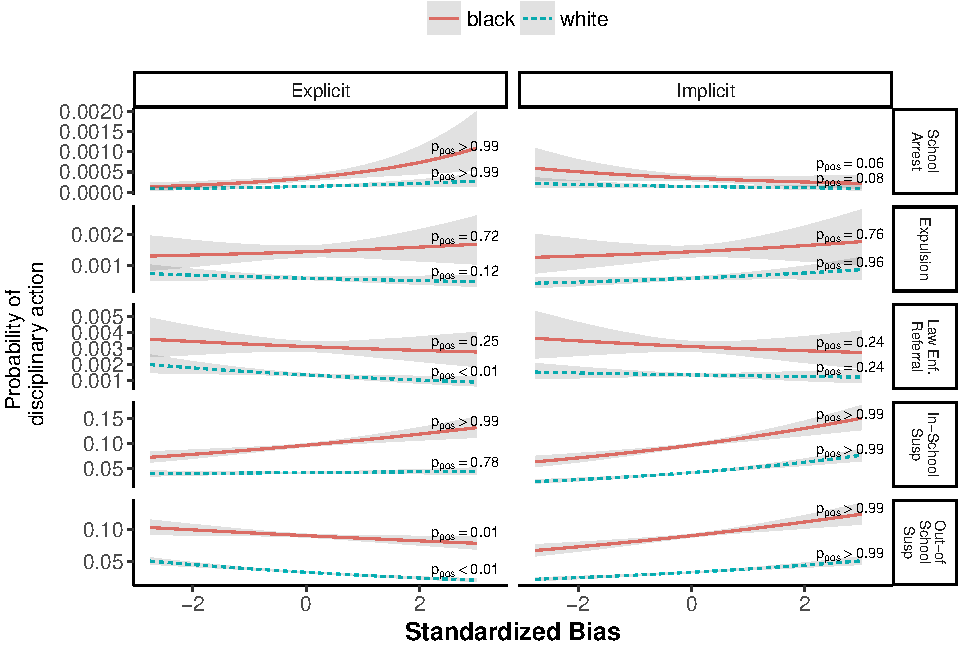
\includegraphics{pnas_supporting_files/figure-latex/disc-probs-1.pdf}
\caption{\label{fig:disc-probs}\label{fig:disc-probs}Association between
bias and the probability of receiving discipline for black and white
students. Lines represent the mean of the posterior. Bands indicate 95\%
uncertainty intervals. Printed p\_\{pos\} represents the posterior
probability that the association is positive.}
\end{figure}

\begin{landscape}\begin{table}

\caption{\label{tab:reg-coefs-sex}\label{tab:reg-coefs-sex}Regression coefficient estimates for the population-level (i.e. fixed) effects, 
             along with 95\% uncertainty intervals for each of the disciplinary metrics. Bias estimates are from sexuality data.}
\centering
\begin{tabular}[t]{llllll}
\toprule
 & Out-of-School Suspension & In-School Suspension & Law Enf. Referral & Expulsion & School-Related Arrest\\
\midrule
Intercept & \textbf{-2.29 [-2.33,-2.26]} & \textbf{-2.23 [-2.27,-2.19]} & \textbf{-5.72 [-5.83,-5.62]} & \textbf{-6.54 [-6.67,-6.41]} & \textbf{-7.98 [-8.2,-7.77]}\\
black-white ratio & \textbf{-0.19 [-0.25,-0.14]} & \textbf{-0.43 [-0.51,-0.36]} & \textbf{0.18 [0.03,0.34]} & -0.11 [-0.32,0.08] & 0.11 [-0.2,0.44]\\
proportion black & \textbf{0.33 [0.26,0.41]} & \textbf{0.44 [0.34,0.54]} & \textbf{-0.42 [-0.62,-0.2]} & -0.16 [-0.42,0.09] & -0.29 [-0.67,0.08]\\
college grads & \textbf{0.05 [0.01,0.09]} & \textbf{-0.05 [-0.1,0]} & \textbf{0.14 [0.02,0.25]} & -0.01 [-0.14,0.12] & \textbf{0.23 [0.04,0.43]}\\
crime & 0.03 [0,0.06] & \textbf{0.06 [0.02,0.1]} & 0.03 [-0.05,0.12] & \textbf{0.14 [0.04,0.23]} & 0.03 [-0.11,0.18]\\
\addlinespace
housing density & \textbf{-0.04 [-0.07,-0.02]} & -0.03 [-0.06,0.01] & 0 [-0.07,0.06] & -0.05 [-0.13,0.03] & \textbf{-0.14 [-0.24,-0.04]}\\
dissimilarity & \textbf{0.17 [0.14,0.21]} & \textbf{0.09 [0.05,0.13]} & \textbf{0.17 [0.08,0.27]} & \textbf{0.29 [0.17,0.41]} & \textbf{0.48 [0.31,0.66]}\\
income & \textbf{-0.08 [-0.13,-0.03]} & -0.03 [-0.09,0.04] & -0.07 [-0.2,0.07] & \textbf{-0.27 [-0.45,-0.09]} & 0.01 [-0.23,0.24]\\
mobility & \textbf{-0.05 [-0.1,-0.02]} & -0.03 [-0.08,0.02] & 0.09 [-0.02,0.2] & -0.01 [-0.16,0.13] & 0 [-0.21,0.21]\\
poverty & -0.02 [-0.1,0.06] & \textbf{0.15 [0.05,0.25]} & \textbf{-0.46 [-0.69,-0.24]} & \textbf{-0.38 [-0.66,-0.1]} & -0.3 [-0.69,0.08]\\
\addlinespace
total population & -0.01 [-0.04,0.02] & -0.02 [-0.06,0.01] & -0.03 [-0.11,0.04] & 0 [-0.08,0.08] & \textbf{0.11 [0.01,0.22]}\\
unemployment & \textbf{0.2 [0.15,0.24]} & 0.04 [-0.01,0.09] & 0.09 [-0.02,0.21] & \textbf{0.21 [0.07,0.35]} & 0.15 [-0.06,0.36]\\
proportion white & 0.03 [-0.04,0.1] & 0.09 [0,0.18] & \textbf{-0.23 [-0.43,-0.03]} & -0.23 [-0.47,0.01] & -0.15 [-0.47,0.17]\\
race: white & \textbf{-1.06 [-1.09,-1.04]} & \textbf{-0.91 [-0.93,-0.88]} & \textbf{-0.86 [-0.94,-0.77]} & \textbf{-0.88 [-0.99,-0.76]} & \textbf{-0.89 [-1.07,-0.7]}\\
implicit bias & 0.05 [0,0.09] & \textbf{0.13 [0.08,0.19]} & 0.02 [-0.1,0.14] & \textbf{0.2 [0.06,0.35]} & \textbf{0.4 [0.18,0.61]}\\
\addlinespace
explicit bias & \textbf{-0.14 [-0.18,-0.1]} & -0.03 [-0.08,0.03] & \textbf{-0.26 [-0.38,-0.14]} & \textbf{-0.15 [-0.29,0]} & \textbf{-0.36 [-0.57,-0.14]}\\
black-white ratio*race: white & \textbf{0.13 [0.08,0.18]} & 0.06 [0,0.12] & \textbf{-0.22 [-0.42,-0.03]} & 0.16 [-0.05,0.37] & -0.2 [-0.6,0.18]\\
proportion black*race: white & \textbf{-0.09 [-0.16,-0.03]} & -0.05 [-0.12,0.01] & 0.13 [-0.05,0.31] & -0.06 [-0.28,0.16] & 0.12 [-0.21,0.46]\\
college grads*race: white & \textbf{-0.12 [-0.15,-0.09]} & \textbf{-0.06 [-0.09,-0.02]} & \textbf{-0.18 [-0.25,-0.1]} & \textbf{-0.13 [-0.23,-0.02]} & -0.09 [-0.22,0.05]\\
crime*race: white & -0.02 [-0.04,0] & 0.01 [-0.02,0.03] & 0.02 [-0.03,0.07] & -0.04 [-0.11,0.03] & 0.05 [-0.04,0.14]\\
\addlinespace
housing density*race: white & \textbf{-0.02 [-0.04,0]} & -0.01 [-0.03,0] & -0.01 [-0.04,0.02] & -0.03 [-0.08,0.02] & -0.06 [-0.22,0.09]\\
dissimilarity*race: white & \textbf{-0.11 [-0.14,-0.08]} & \textbf{-0.05 [-0.07,-0.02]} & \textbf{-0.09 [-0.15,-0.02]} & -0.04 [-0.13,0.05] & \textbf{-0.2 [-0.33,-0.08]}\\
income*race: white & \textbf{-0.06 [-0.09,-0.02]} & \textbf{-0.09 [-0.13,-0.05]} & -0.06 [-0.15,0.02] & 0.03 [-0.1,0.16] & -0.1 [-0.25,0.05]\\
mobility*race: white & 0.03 [0,0.07] & 0.01 [-0.03,0.04] & -0.04 [-0.13,0.05] & -0.01 [-0.13,0.12] & 0.05 [-0.12,0.22]\\
poverty*race: white & 0.05 [-0.01,0.11] & 0 [-0.06,0.06] & -0.09 [-0.24,0.07] & 0.02 [-0.2,0.24] & -0.05 [-0.32,0.23]\\
\addlinespace
total population*race: white & \textbf{-0.03 [-0.05,-0.01]} & -0.01 [-0.03,0.01] & 0 [-0.04,0.03] & -0.02 [-0.06,0.03] & -0.01 [-0.05,0.04]\\
unemployment*race: white & 0 [-0.03,0.03] & 0.01 [-0.02,0.04] & -0.02 [-0.1,0.06] & 0.04 [-0.06,0.15] & -0.01 [-0.16,0.13]\\
proportion white*race: white & 0.01 [-0.05,0.07] & 0.01 [-0.05,0.07] & -0.1 [-0.23,0.03] & 0.06 [-0.12,0.25] & -0.07 [-0.28,0.14]\\
implicit bias*race: white & -0.01 [-0.05,0.02] & -0.01 [-0.04,0.02] & \textbf{-0.11 [-0.19,-0.03]} & 0.05 [-0.06,0.16] & -0.1 [-0.24,0.03]\\
explicit bias*race: white & 0 [-0.03,0.03] & -0.01 [-0.04,0.02] & 0.08 [0,0.16] & -0.03 [-0.14,0.07] & 0.08 [-0.07,0.22]\\
\bottomrule
\end{tabular}
\end{table}
\end{landscape}

\begin{landscape}\begin{table}

\caption{\label{tab:cor-tab}\label{tab:cor-tab}Correlation matrix for all county-level predictor variables.}
\centering
\resizebox{\linewidth}{!}{\begin{tabular}[t]{lllllllllllllllllll}
\toprule
 & 1 & 2 & 3 & 4 & 5 & 6 & 7 & 8 & 9 & 10 & 11 & 12 & 13 & 14 & 15 & 16 & 17 & 18\\
\midrule
1) Implicit Race &  &  &  &  &  &  &  &  &  &  &  &  &  &  &  &  &  & \\
2) Explicit Race & 0.79 &  &  &  &  &  &  &  &  &  &  &  &  &  &  &  &  & \\
3) Implicit Sex & 0.51 & 0.58 &  &  &  &  &  &  &  &  &  &  &  &  &  &  &  & \\
4) Explicit Sex & 0.3 & 0.44 & 0.76 &  &  &  &  &  &  &  &  &  &  &  &  &  &  & \\
5) Population Size & 0.02 & -0.04 & -0.23 & -0.24 &  &  &  &  &  &  &  &  &  &  &  &  &  & \\
6) White Population & 0.01 & -0.05 & -0.25 & -0.26 & 0.98 &  &  &  &  &  &  &  &  &  &  &  &  & \\
7) Black Population & 0.11 & 0.06 & -0.13 & -0.16 & 0.78 & 0.71 &  &  &  &  &  &  &  &  &  &  &  & \\
8) College Grads & -0.11 & -0.09 & -0.33 & -0.29 & 0.22 & 0.24 & 0.19 &  &  &  &  &  &  &  &  &  &  & \\
9) Unemployment & 0.28 & 0.13 & 0.07 & -0.02 & 0.14 & 0.13 & 0.18 & -0.19 &  &  &  &  &  &  &  &  &  & \\
10) Income & -0.21 & -0.18 & -0.38 & -0.36 & 0.24 & 0.28 & 0.11 & 0.43 & -0.24 &  &  &  &  &  &  &  &  & \\
11) Poverty & 0.34 & 0.26 & 0.33 & 0.29 & -0.04 & -0.07 & 0.05 & -0.37 & 0.51 & -0.71 &  &  &  &  &  &  &  & \\
12) Crime & 0.12 & 0.05 & -0.08 & -0.08 & 0.13 & 0.11 & 0.15 & -0.07 & 0.31 & -0.1 & 0.26 &  &  &  &  &  &  & \\
13) Housing Density & 0 & -0.06 & -0.18 & -0.16 & 0.3 & 0.25 & 0.39 & 0.23 & 0.06 & 0.13 & 0.01 & 0.1 &  &  &  &  &  & \\
14) Mobility & -0.25 & -0.19 & -0.1 & -0.06 & -0.1 & -0.1 & -0.11 & -0.03 & -0.14 & 0.03 & -0.12 & -0.09 & -0.05 &  &  &  &  & \\
15) Proportion White & -0.37 & -0.32 & -0.13 & -0.07 & -0.19 & -0.14 & -0.3 & 0.08 & -0.5 & 0.14 & -0.53 & -0.38 & -0.15 & 0.21 &  &  &  & \\
16) Proportion Black & 0.58 & 0.52 & 0.32 & 0.2 & 0.08 & 0.04 & 0.26 & -0.08 & 0.4 & -0.26 & 0.5 & 0.28 & 0.09 & -0.24 & -0.81 &  &  & \\
17) Black-White Ratio & 0.42 & 0.38 & 0.27 & 0.17 & 0.04 & 0 & 0.21 & -0.07 & 0.36 & -0.25 & 0.48 & 0.24 & 0.07 & -0.17 & -0.73 & 0.89 &  & \\
18) Segregation & -0.04 & -0.07 & -0.13 & -0.15 & 0.18 & 0.2 & 0.17 & 0.05 & 0.16 & 0.07 & -0.02 & 0.06 & 0.1 & 0.09 & 0.08 & -0.1 & -0.09 & \\
\addlinespace[.5em]
\multicolumn{19}{l}{\textbf{}}\\
\hspace{1em}Mean & 0.4 & 0.83 & 0.38 & 1.65 & 99.93 & 73.75 & 12.6 & 6.08 & 4.94 & 46.55 & 12.35 & 1.1 & 113.43 & 14.89 & 0.84 & 0.09 & 0.17 & 0.38\\
\hspace{1em}SD & 0.02 & 0.17 & 0.05 & 0.49 & 319.97 & 200.81 & 54.76 & 4.87 & 1.99 & 12.08 & 5.68 & 0.94 & 823.84 & 17.69 & 0.17 & 0.14 & 0.42 & 0.19\\
\bottomrule
\multicolumn{19}{l}{\textsuperscript{1} Crime rate is scaled to rate per 1000 people}\\
\multicolumn{19}{l}{\textsuperscript{2} Total population, black population, and white population are in 1000's of people}\\
\multicolumn{19}{l}{\textsuperscript{3} Income is in 1000's of dollars}\\
\end{tabular}}
\end{table}
\end{landscape}


\end{document}
